\chapter{Fabrication d'un transistor moléculaire}

L'une des étapes essentielles dans la caractérisation d'un aimant moléculaire consiste a fabriquer un transistor à molécule unique~(SMT - Single Molecule Transistor). Du fait de la petite taille de ces dernières~($1\,nm$ environ), il est impossible de faire appel à des techniques lithographiques classiques. Nous avons déjà abordé les différentes solutions développées dans le cadre de la spintronique. Nous avons fait le choix d'utiliser la technique d'électromigration développé par H. Park \textit{et al.} avec quelques adaptations.

Deux éléments sont prépondérants dans la qualité d'un SMT : l’efficacité de la grille et la bonne qualité des interstices. Nous présenterons dans une première partie les différentes étapes nous permettant d'obtenir une grille efficace, après avoir défini les critères définissant cette efficacité. Ensuite, nous montrerons comment il est possible, en utilisant le phénomène d'électromigration, de produire des interstices nanométriques. Nous verrons enfin la technique de déposition ainsi que les premières étapes de caractérisation électrique des dispositifs obtenus.


\begin{figure}
\parbox{6.5cm}{
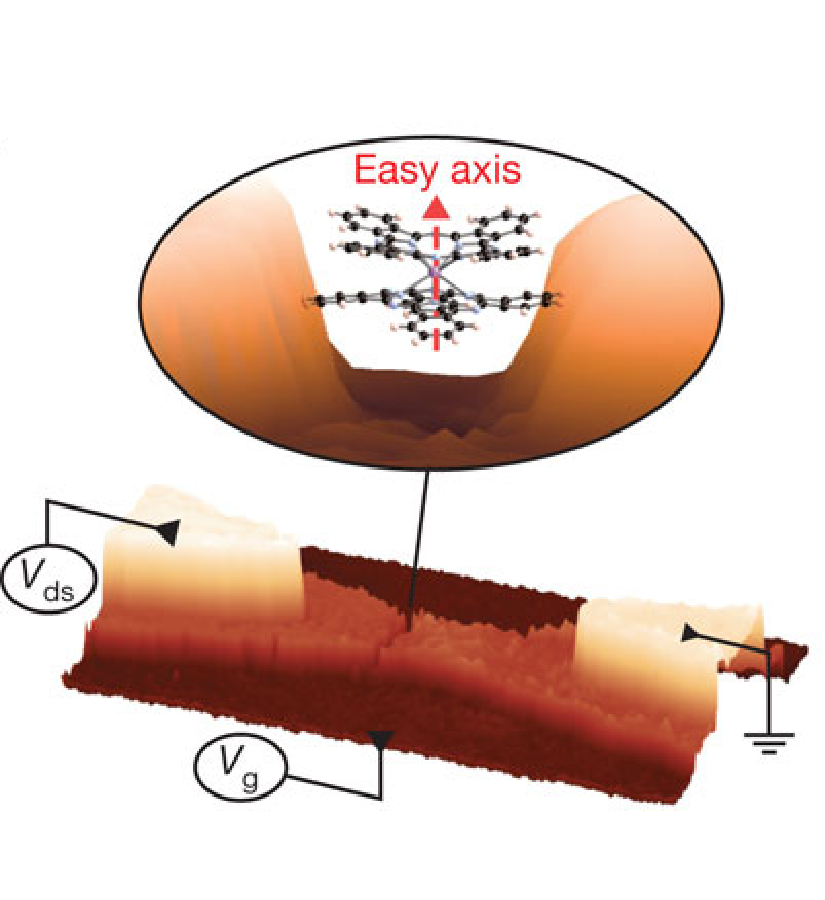
\includegraphics[scale=0.45]{Fabrication/ImageTrans/ImageTrans.pdf} 
}
\parbox{7cm}{\caption{Extrapolation 3D d'une image obtenue par microscopie électronique à balayage. Elle correspond à la structure finale que l'on souhaite obtenir : les électrodes de source et de drain, l'électrode de grille, ainsi qu'un interstice nanométrique dans lequel une molécule est piégée~(extrait de~\cite{Vincent2012}).}
\label{ImageTrans}
}
\end{figure}

\section{Réalisation d'une grille locale}
La grille est un élément essentiel du transistor et c'est également vrai d'un transistor moléculaire~\cite{Datta2009,Zant2006}. Dans ce dernier cas, elle permet notamment de moduler le potentiel chimique de la molécule allant jusqu'à modifier son état de charge~\cite{Beenakker1991,Wiel2002,Hanson2007}~(cf annexe sur le transport mésoscopique). Elle permet également de contrôler la conductance du système~(avec le concours de la tension source-drain), et donc de choisir des points de fonctionnement adaptés. Nous détaillerons ce dernier point dans le chapitre résultat. 

L'efficacité intrinsèque d'une grille peut être résumée en un seul critère~:~la charge induite. Celle-ci s'exprime simplement par $Q = CV_g^{max}$ où $Q$ est le charge induite et $C$ est la capacité associée à la grille, $V_g^{max}$ étant la tension maximale applicable à la grille. Elle dépend essentiellement de trois paramètres physiques : le champ électrique maximum applicable, l'épaisseur et la permittivité de l'oxyde ~\cite{Biercuk2003}. 

Outre les paramètres que l'on vient de voir, il existe plusieurs géométries de grille susceptibles d'avoir une influence sur l’efficacité de cette dernière. On peut identifier trois géométries : la grille au-dessus ou  ``\textit{top-gate}'', la grille latérale et la grille arrière ou  ``\textit{back-gate}''.

\subsection{Les différentes géométries}
Je ne donnerai ici qu'un rapide présentation des différents grilles existantes. Pour une comparaison plus détaillé entre ces différentes géométrie est disponible dans la thèse de ??.
\subsubsection{La ``\textit{top-gate"}}
Cette configuration est utilisée dans l'industrie en ce qui concerne les transistors à effet de champ conventionnels. On la retrouve également dans les dispositifs expérimentaux faisant appel à des nanofils~\cite{Fasth2005} ou bien encore à des nanotubes~\cite{Javey2002}. Elle a également pu être implémentée dans le cas de nanotubes suspendus donnant des résultats plus que convaincant~\cite{Leturcq2009}.

Cette configuration est cependant difficilement compatible avec l'électromigration. En effet, dans ce cas, le gap formant la source et le drain se fait après les étapes de lithographie, ce qui serait impossible si le fil d'or était recouvert par une grille. Pour produire une grille compatible avec l'électromigration, il faut se tourner vers d'autres géométries comme la configuration latérale.

\subsubsection{La grille latérale}
Cette configuration consiste à placer la grille latéralement vis à vis du gap obtenu par électromigration~\cite{Mangin2009}. De plus, accompagnée d'une grille arrière, elle permet d'avoir deux moyens d'action sur le potentiel chimique de la molécule située dans la gap. 

Il est en revanche très difficile de contr\^oler précisément la position de cette grille et elle se trouve donc souvent située à plusieurs dizaines de nanomètres du gap. De plus, le r\^ole de l'oxyde est, dans ce cas, joué par l'air qui possède une permittivité proche de l'unité. Cette configuration abouti donc, de manière générale, à une grille moins efficace que la configuration grille arrière~\cite{Aurore2009} que nous allons voir maintenant.


\subsubsection{La grille arrière}
Dans cette configuration, la grille se situe sous le dispositif. Cette configuration a notamment été adoptée pour la réalisation du premier transistor à molécule unique~\cite{Park2000}. Elle est bien s\^ur compatible avec l'électromigration et, implémentée en grille locale, elle permet d'obtenir des grilles très efficaces. Pour ces raison, nous avons choisie d’adopter cette configuration pour nos échantillons. De plus, sa fabrication peut \^etre grandement facilitée par l'utilisation de la technique ALD que nous allons présenter dans la suite.


\subsection{Création de l'électrode de grille}

La première étape de la fabrication de notre grille locale consiste en l'obtention de l'électrode de grille. Compte tenu des tailles caractéristiques de cette dernière, cette électrode peut \^etre obtenu à l'aide d'une lithographie optique ultra-violet profond (DUV - Deep Ulta-Violet). A cette fin, une méthode bicouche LOR3A/UV3 est utilisée en suivant les instructions du Tab.\ref{tab_recette}, avec pour seule différence, l'épaisseur d'or déposé : $20\,nm$.

\begin{table}
\begin{center}
\begin{tabular}{|p{0.5cm}|p{4cm}|p{4cm}|p{3cm}|}
  \hline
\,& \textbf{étape} & \textbf{procédé} & \textbf{paramètres} \tabularnewline
\hline
1 &  nettoyage du wafer & acétone, ethanol, isopropanol et plasma oxygène (RIE)& $2\,$min \tabularnewline
\hline
 2 & étalement de LOR 3A pour une épaisseur de $400\,$nm& tournette & v\,:\,$2000\,$tr.min$^{-1}$, a\,:\,$2000\,$tr.min$^{-2}$, t\,:\,$30\,$s \tabularnewline
\hline
 3 & cuisson & plaque chauffante & $1\,$min à $170\,\degres$C \tabularnewline
\hline
4 & étalement de UV3 & tournette & v\,:\,$4000\,$tr.min$^{-1}$, a\,:\,$2000\,$tr.min$^{-2}$, t\,:\,$30\,$s \tabularnewline
\hline
5 & cuisson & plaque chauffante & $1\,$min à $130\,\degres$C \tabularnewline
\hline
6 & insolation & aligneur dUV MJB3 & $5.5\,$s à $0.3\,$mW.cm$^{-2}$\tabularnewline
\hline
7 & recuisson & plaque chauffante & $1\,$min à $130\,\degres$C \tabularnewline
\hline
8 & développement & MF-CD-26 & $30-40\,$s\tabularnewline
\hline
9 & neutralisation du développeur & eau DI & $1\,$min\tabularnewline
\hline
10 & dépôt de la couche d'accroche métallique & évaporateur à canon à électron PLASSYS & $5\,$nm de Ti à $0.1\,$nm.s$^{-1}$ \tabularnewline
\hline
11 & dépôt de la couche métallique principale & évaporateur à canon à électron PLASSYS & $100\,$nm de Au à $0.1\,$nm.s$^{-1}$ \tabularnewline
\hline
12 & \textit{lift-off} & acétone & $10\,$min à $1\,$h, on peut l'assister par ultra-son à $80\%$ de la puissance maximum. \tabularnewline
\hline
 13 & dissolution de LOR3A & PG-Remover & $1\,$h à $80\,\degres$C \tabularnewline
\hline
14 & rinçage & acétone et isopropanol & $1\,$min de chaque sous la pissette\tabularnewline
\hline
15 & séchage & azote sec & wafer posé sur du papier absorbant, pistolet à la verticale du wafer, ne pas toucher le wafer avec des pinces\tabularnewline
\hline
16 & nettoyage & plasma oxygène (RIE)& $10\,$min\tabularnewline
\hline
\end{tabular}
\caption{Recette du double couche LOR3A/UV3 : celle-ci permet de ne plus avoir d'effet de bord lors des lift-off.}
\label{tab_recette}
\end{center}
\end{table}


Cette étape permet également d'obtenir les marques d'alignements nécessaire à la fabrication des lignes d'amenés. Une première série de marques~(cf carré bleu de la Fig.??) permet d'effectuer un alignement grossier. Ce dernier est ensuite affiné à l'aide d'une deuxième série de repères~(cf carré vert de la Fig??).

La technique bicouche a été préféré à la technique usuelle monocouche, car elle a l'avantage de prévenir la formation de bords lors de l'étape de lift-off~(cf Fig.\ref{lift-off}) qui pourraient entraîner une perte de contact entre la jonction et le plot correspondant lors du passage de marche~(i.e. lorsque la ligne d'amené passe de la surface de silicium à la grille, la hauteur de marche étant donnée par l'épaisseur de la grille).


\begin{figure}
\centering 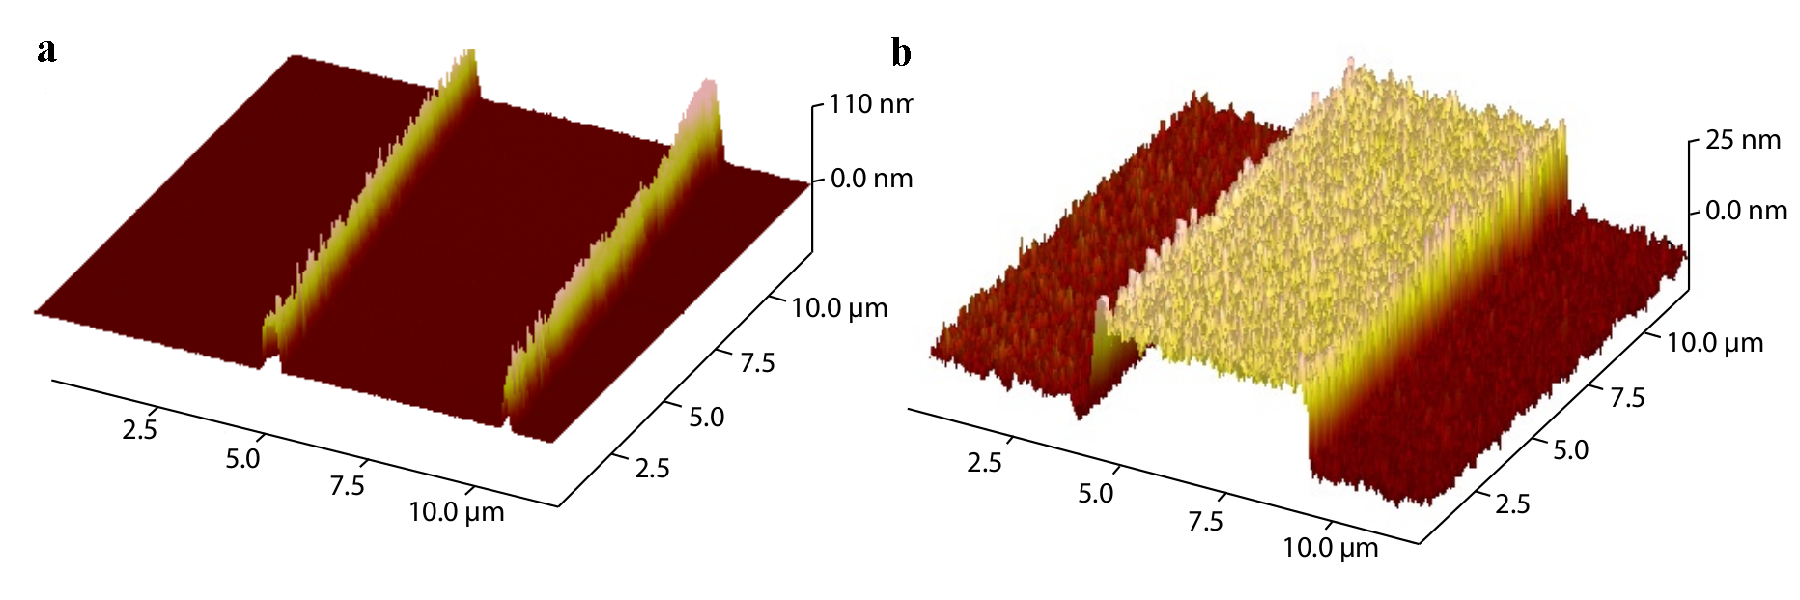
\includegraphics[scale=0.45]{Fabrication/BatmanGrille/BatmanGrille.pdf}
\caption{\textbf{a} : image AFM d'une électrode de grille présentant des bords trop relevés d\^u fait d'un problème de lift-off. \textbf{b} : image AFM montrant une électrode de grille après lift-off ne présentant pas d'anomalie après lift-off~(extrait de~\cite{RochPhD}).}
\label{lift-off}
\end{figure}

Cette première étape est suivie du dépôt d'oxyde par une méthode de dépôt par couche atomique ou ALD~(Atomic Layer Déposition) que nous allons détailler maintenant.

\subsection{Le dép\^ot par ALD}

Comme nous l'avons déjà précisé en introduction, le choix de l'oxyde est très important et, en particulier, la permittivité de ce dernier doit être la plus élevée possible.

Parmi les oxydes à haute permittivité, les plus couramment utilisés sont l'alumine~($\kappa \sim 8$), l'hafnia~($\kappa \sim 17$) et l'oxyde de zirconium~($\kappa \sim 26$)~\cite{Biercuk2003}. De manière générale, le premier est obtenu par dépôt d'une électrode d'aluminium, puis exposition à une atmosphère riche en oxygène ou bien par ALD. Les deux derniers sont en général obtenus par ALD ou, plus rarement, par MOCVD~(Metalorganic Chemical Vapour Deposition). Lorsque je suis arrivé en thèse, la technique par oxydation naturelle était en usage. Bien que relativement facile à mettre en œuvre, il est difficile de connaître avec exactitude l'épaisseur d'oxyde. De plus, nous avons observé une grande variabilité dans la qualité des grilles obtenues par ce procédé.

Nous avons donc développé un nouveau procédé inspiré de~\cite{Biercuk2003} , en utilisant une méthode ALD, nous permettant d'obtenir une grille avec un oxyde de $8\,nm$ environs. Parmi les trois oxydes précédemment cités, nous avons choisi l'oxyde d'hafnium. Celui si à l'avantage d'être fortement documenté et présente des performances supérieures à l'alumine pour ce qui est de la charge induite~\cite{Biercuk2003}. 

La technique d'ALD originellement appelée ALE~(pour Atomic Layer Epitaxie) a été breveté dans les années 1970 et remise au goût du jour pour les besoins toujours plus grands de la microélectronique~\cite{Leskelae2003}. Elle consiste en une succession de deux réactions auto-limitantes, aboutissant à la formation d'un oxyde comme le montre la Fig.\ref{ALD}.

\begin{figure}
\centering 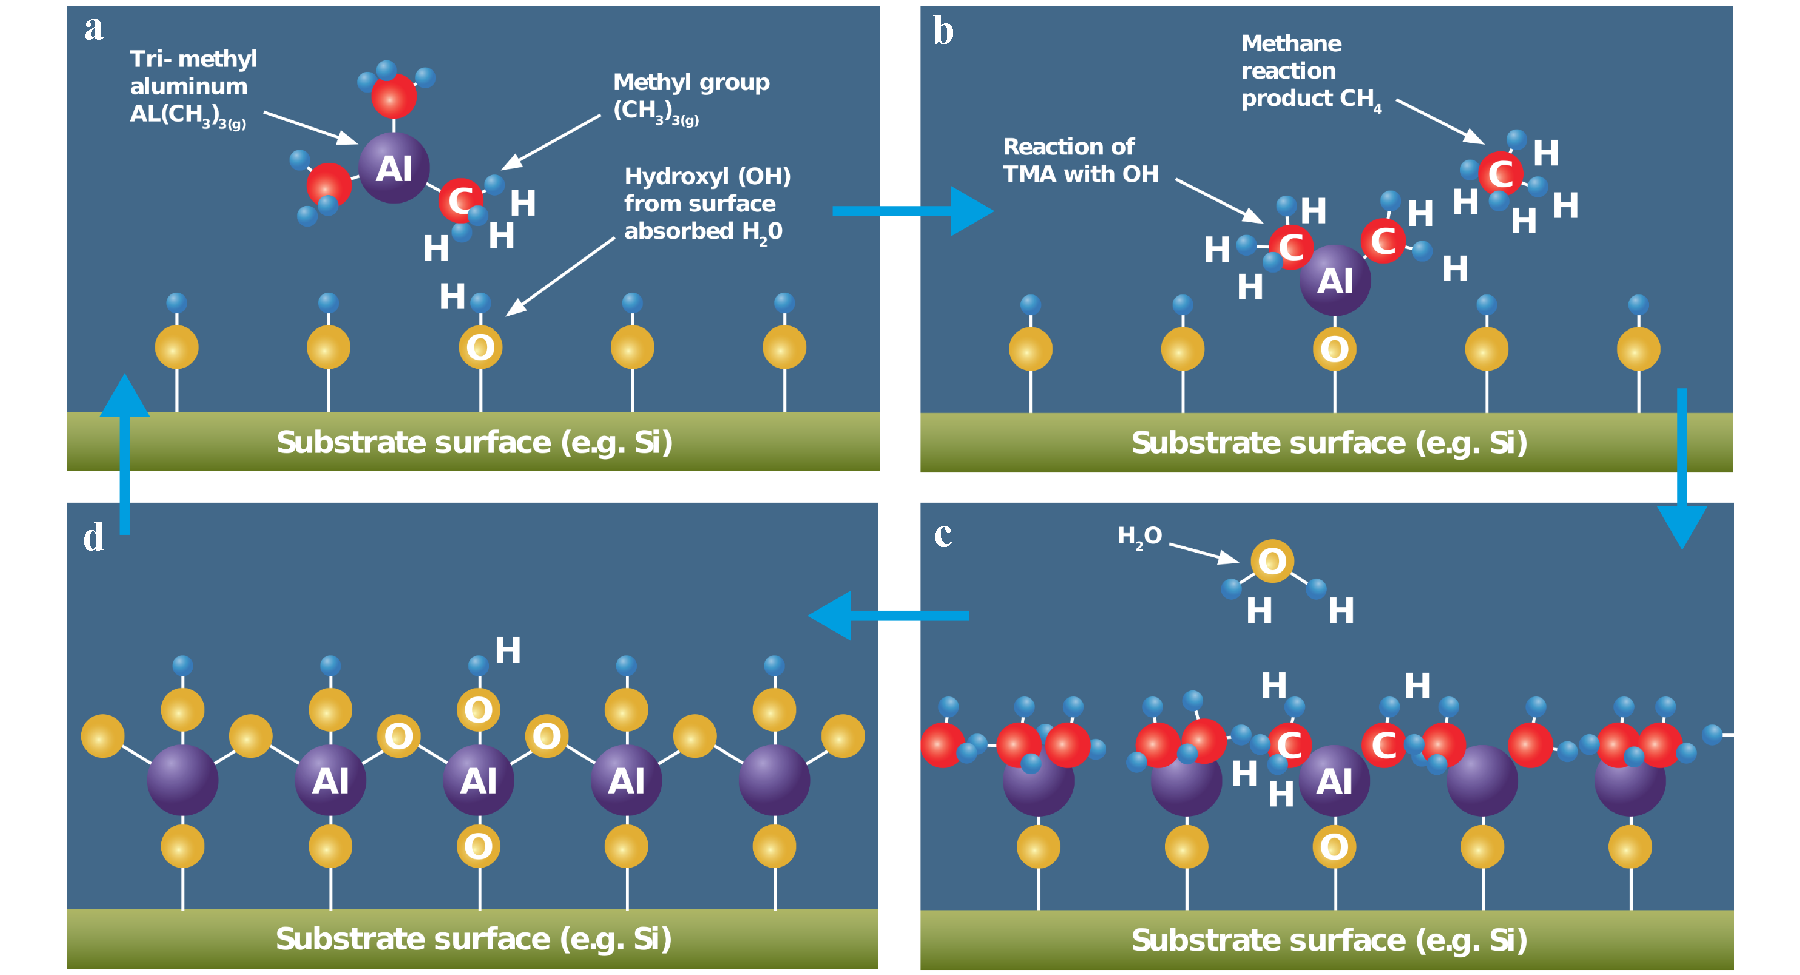
\includegraphics[scale=0.45]{Fabrication/ALD/ALD.pdf}
\caption{Première étape du cycle ALD : le premier précurseur, ici du Al(CH$_3$)$_{3(g)}$, se fixe à la surface~(\textbf{a}) et le produit issue la réaction de fixation sont évacués par un flux de gaz inerte~(\textbf{b}). Dans un deuxième temps, de l'eau est injecté et réagi avec la première couche de précurseur~(\textbf{c}) pour former une couche atomique d'oxyde~(\textbf{d}). Le cycle se répère ensuite à raison d'une couche atomique par cycle. (extrait du site CambrigeNanoTech)}
\label{ALD}
\end{figure}


Le premier avantage de la technique est sa facilité de mise en œuvre. Le contrôle du procédé, couche par couche, permet de choisir l'épaisseur d'oxyde déposé avec une grande précision. De plus, la nature de ce dernier est uniquement déterminée par les précurseurs utilisés, ce qui donne un large choix de matériaux. Afin d'obtenir un oxyde de qualité pour les applications électroniques, celui-ci doit remplir deux critères : il doit contenir peu d'impuretés et être de préférence amorphe~\cite{Kim2003}.

\begin{table}
\begin{center}
\begin{tabular}{|p{0.5cm}|p{6cm}|p{6cm}|}
\hline
\multicolumn{3}{|c|}{\textbf{Réglages}} \tabularnewline
\hline
\multicolumn{2}{|l|}{\textbf{élement}} & \textbf{paramètres} \tabularnewline
\hline
\multicolumn{2}{|l|}{température du précurseur} & $90\, \degres C$ \tabularnewline
\hline
\multicolumn{2}{|l|}{température du \textit{Tee}} & $150\, \degres C$ \tabularnewline
\hline
\multicolumn{2}{|l|}{température de la chambre~(\textit{inner} et \textit{outer})} & $100\, \degres C$ \tabularnewline
\hline
\multicolumn{2}{|l|}{température du \textit{Bellow}} & $150\, \degres C$ \tabularnewline
\hline
\multicolumn{2}{|l|}{\multirow{2}{*}{flux d'azote}} & $20\, sccm$ \newline (pression d'environs $0.5\,Torr$) \tabularnewline
\hline
\hline
\multicolumn{3}{|c|}{\textbf{Procédé}} \tabularnewline
\hline
\,& \textbf{étape} & \textbf{paramètres} \tabularnewline
\hline
1 & pluse de TDMAH & $0.015\,s$ \tabularnewline
\hline
2 & temps d'attente & $120\,s$ \tabularnewline
\hline
3 & pulse d'eau & $0.015\,s$ \tabularnewline
\hline
4 & temps d'attente & $120\,s$ \tabularnewline
\hline
\end{tabular}
\caption{Paramètres et réglages du procédé ALD.}
\label{recette_ALD}
\end{center}
\end{table}



Pour remplir le premier critère, l'idéal est de chauffer de façon suffisante le substrat afin de désorber efficacement les déchets produits lors de la fixation du précurseur~(cf Fig.\ref{ALD}). Afin d'obtenir une structure amorphe, il est, au contraire, préférable d'effectuer le dép\^ot à basse température~\cite{Triyoso2004}, ce qui a également l'avantage de rendre le procédé compatible avec une étape de lithographie~\cite{Biercuk2003}~(évitant à la résine de brûler) et de diminuer la rugosité de l'oxyde~\cite{Triyoso2004}. Il faut donc arriver à trouver un compromis entre ces deux conditions contradictoires.

Celui-ci été trouvé en laissant un délai conséquent entre les différentes étapes du dépôt, permettant aux produits de réaction de désorber~\cite{Biercuk2003}. Cela se traduit par un temps d'attente entre chaque étape de cycle de 2 minutes. Un dépôt de $8\,nm$~(environs 80\,cycles) d'hafnia prend donc un peu plus de cinq heures~(pour les détails concernant le dépôt ALD, le lecteur peut se référer au Tab.\ref{recette_ALD}). Si ce temps peut paraître long au premier abord, il ne représente qu'un temps négligeable au regard des autres étapes, et notamment, celle de lithographie électronique que nous allons aborder maintenant.

\begin{figure}
\centering 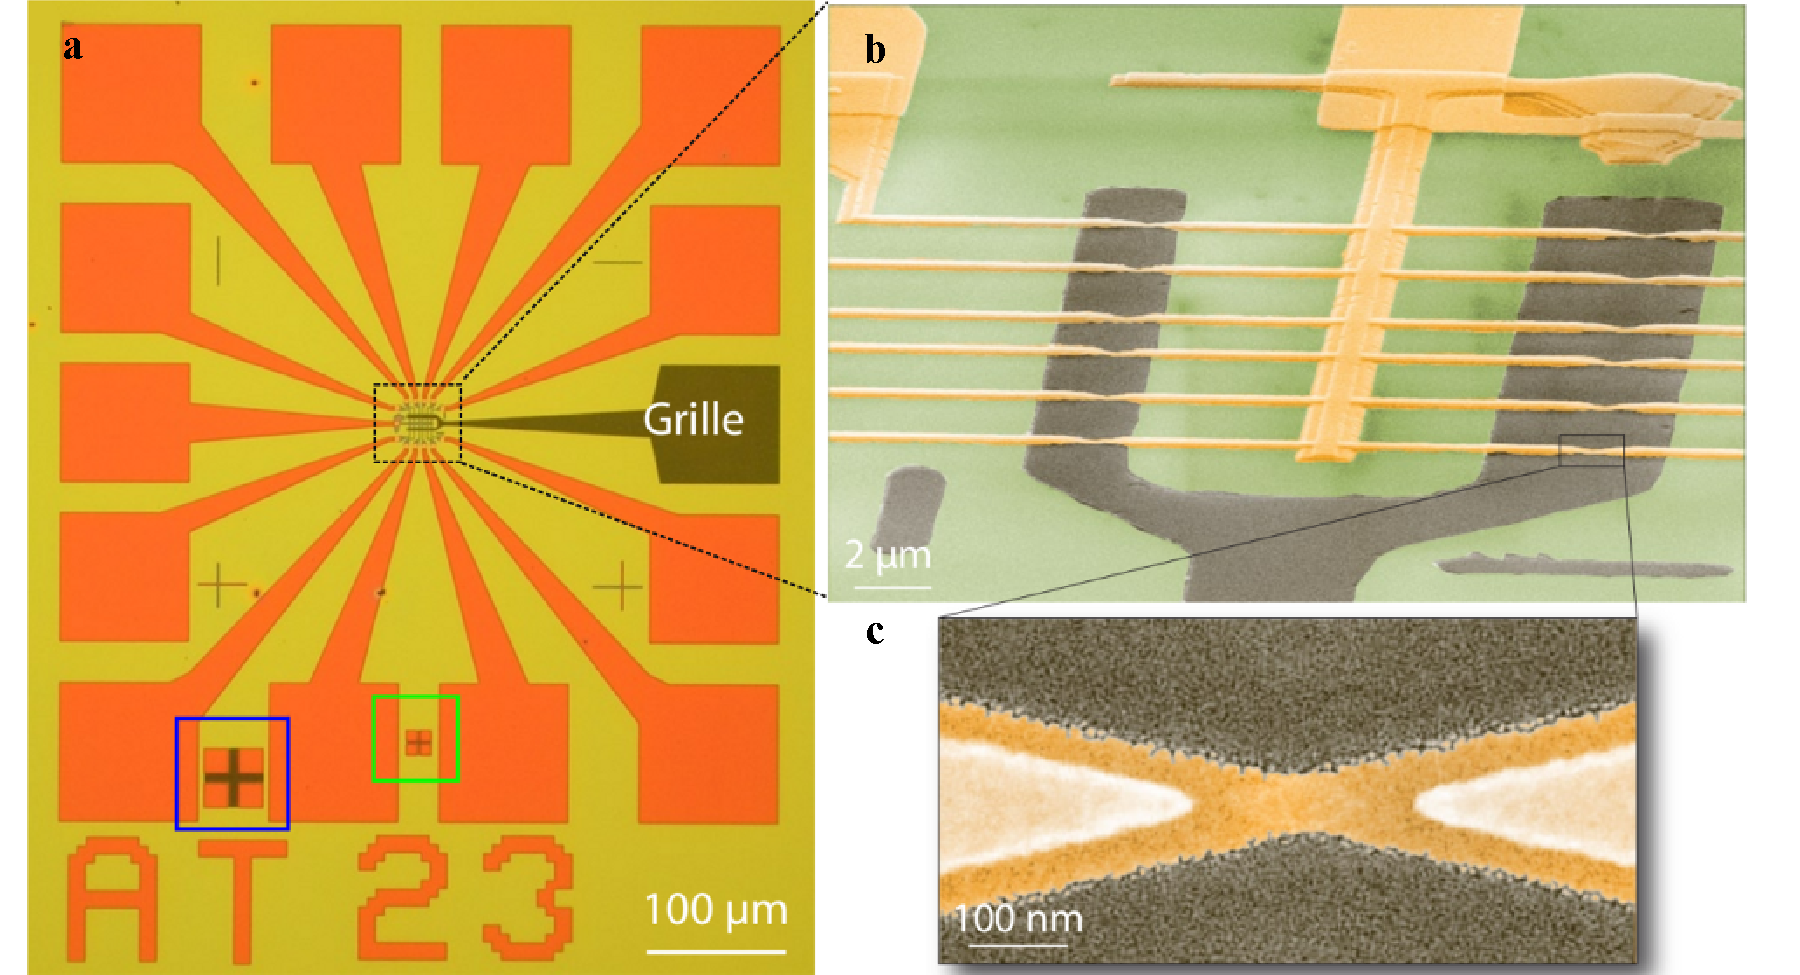
\includegraphics[scale=0.45]{Fabrication/FinalResult/FinalResult.pdf}
\caption{\textbf{a} : Échantillon après les deux étapes de lithographie optique. Les lignes d'amené de courant sont visibles en orange et la grille locale en gris. Les deux carrés repèrent les marques d'alignement. \textbf{b} : Image obtenu par microscopie électronique à balayage montrant la structure centrale de nos échantillons. \textbf{c} grossissement présentant une constriction obtenue à l'aide de l'évaporation sous angle. La grille, colorée en gris, est clairement visible au centre (extrait de \cite{RochPhD}).}
\label{FinalResult}
\end{figure}


%\begin{figure}
%\parbox{6.5cm}{
%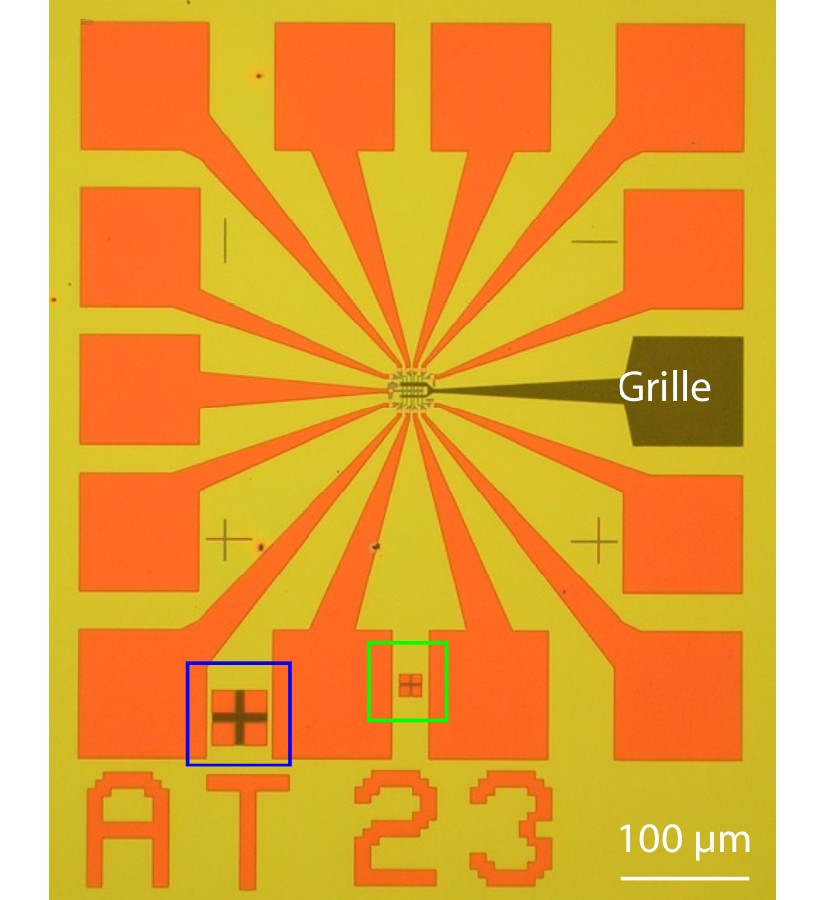
\includegraphics[scale=0.45]{Fabrication/LithoOptique/LithoOptique.pdf} 
%}
%\parbox{7cm}{\caption{Échantillon après les deux étapes de lithographie optique. Les lignes d'amené de courant sont visibles en orange et la grille locale en gris. Les deux carrés repèrent les marques d'alignement~(extrait de~\cite{RochPhD}).}
%\label{LithoOptique}
%}
%\end{figure}




\section{Réalisation d'un nanofil}

\subsection{Lithographie optique}

La seconde étape de lithographie vise à fabriquer les plots d'or nécessaires à la micro-soudure de notre échantillon, ainsi que les lignes d'amené de courant~(cf partie orange de la Fig.\ref{LithoOptique}). La recette du Tab.\ref{tab_recette}  est utilisée pour obtenir un dép\^ot de 100$\,nm$ d'or avec une couche d'accroche en titane. 


Le résultat final est présenté dans la Fig.\ref{LithoOptique} où la partie orange désigne les lignes d'amené de courant et la partie grise la grille locale. La partie centrale va venir accueillir les nanofils d'or comme nous allons le voir dans la suite.


\subsection{Lithographie électronique}



Comme nous l'avons présenté dans l'introduction, notre méthode de fabrication repose sur la technique d'électromigration. Cette dernière, pour fonctionner correctement, a besoin d'\^etre opérée sur des fils d'or très fins, présentant une section de quelques dizaines de nanomètres pour une épaisseur de quelques nanomètres en ce qui concerne la partie la plus fine~(cf Fig.\ref{EvapAngle}). 

\begin{figure}[h!]
\centering 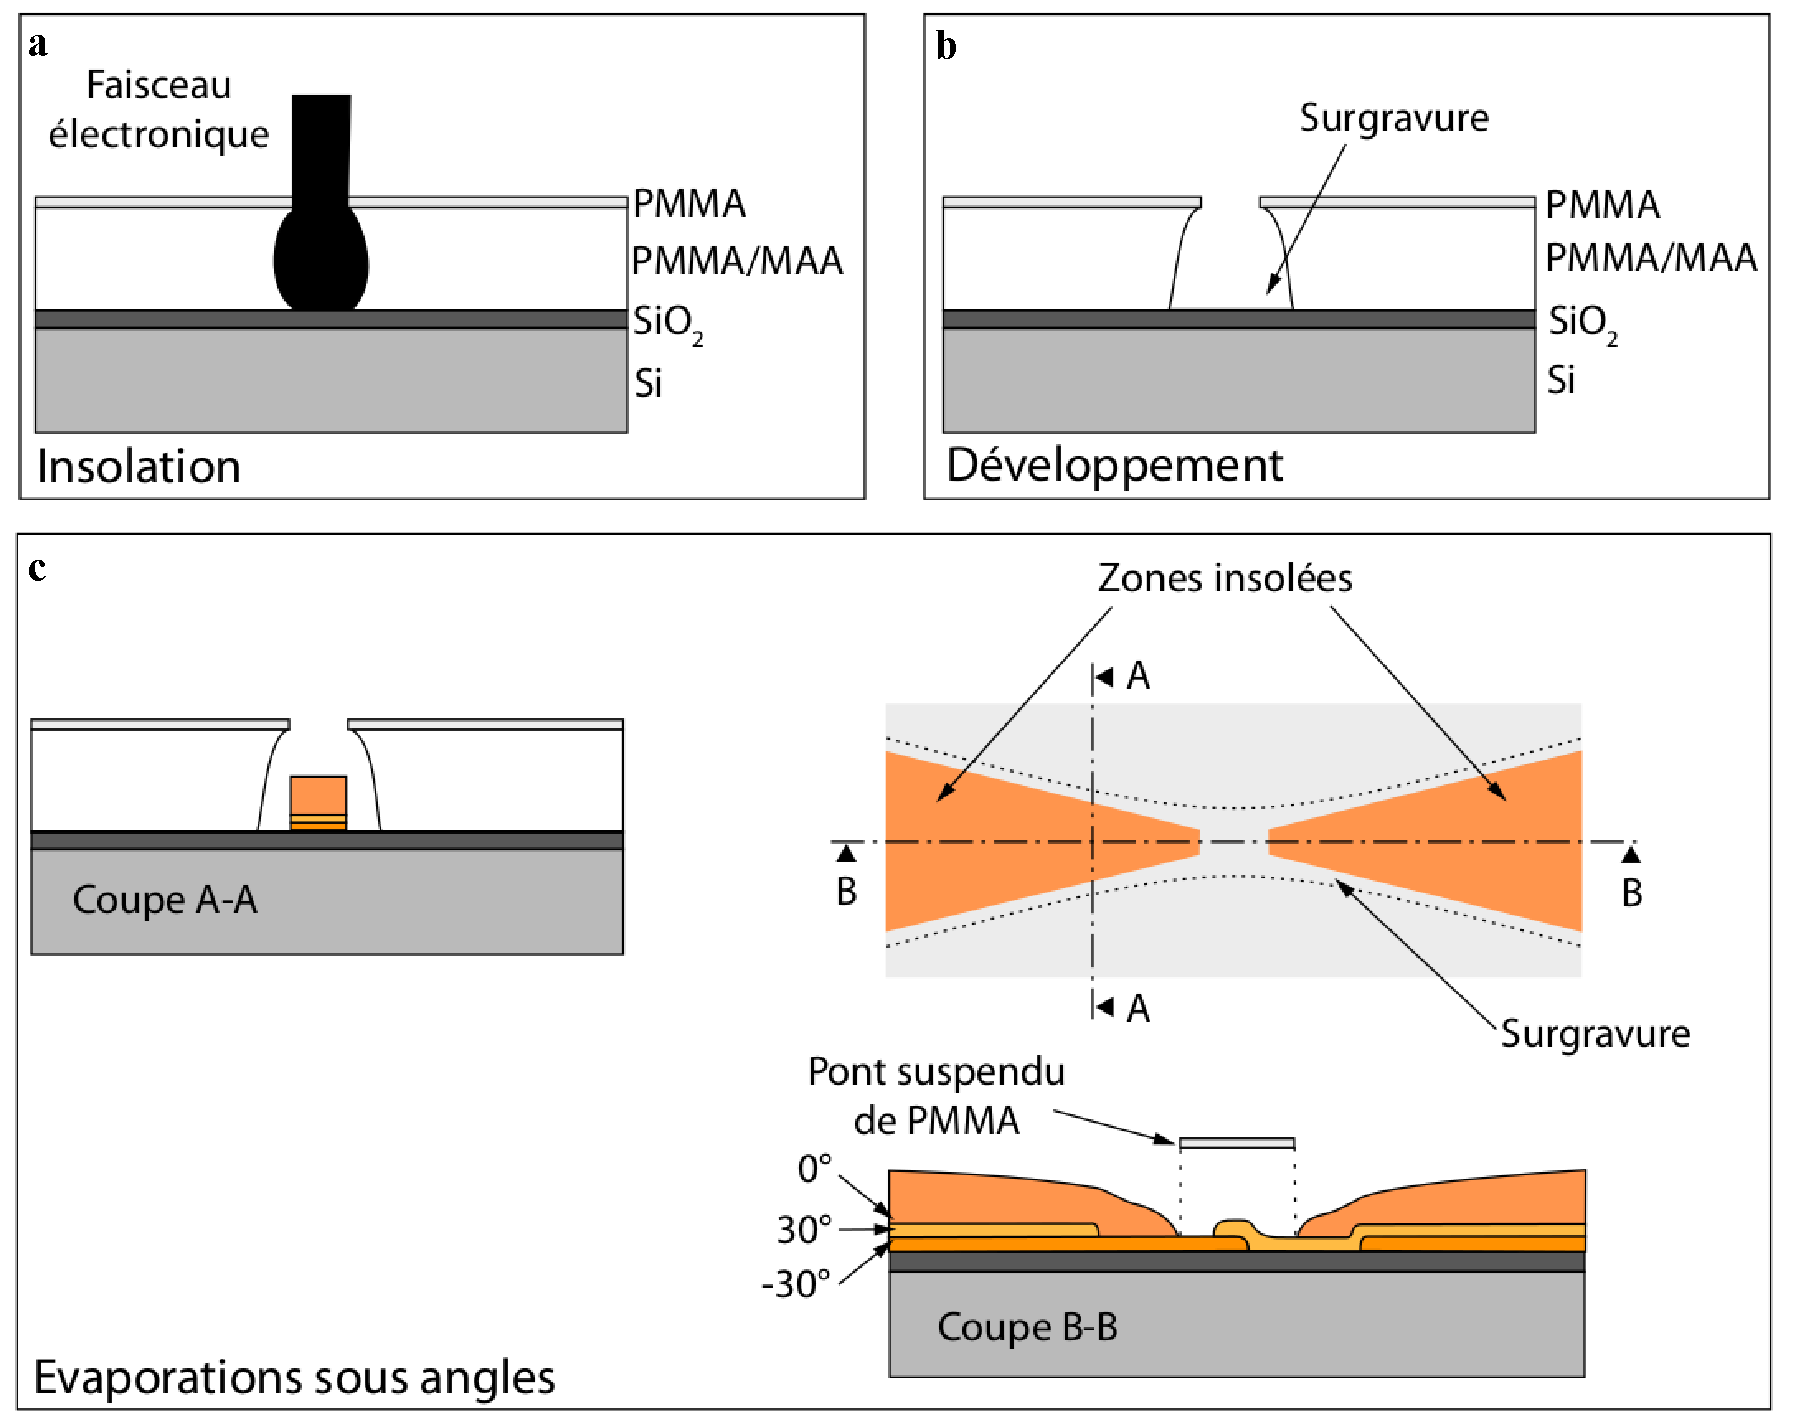
\includegraphics[scale=0.45]{Fabrication/EvapAngle/EvapAngle.pdf}
\caption{\textbf{a} : Insolation par lithographie électronique de la bicouche de résine. La partie la plus proche du substrat~(PMMA/MAA) se trouve plus insolé depart une plus grande sensibilité aux électrons et la présence des électrons rétrodiffusés. \textbf{b} : résultats après développement montrant clairement la surgravure généré par la surexposition de la partie basse. \textbf{c} : Evaporation sous angle : différentes couleurs représente les différents angle d'évaporation (-30$\,\degres$, 0$\,\degres$ et 30$\,\degres$ - extrait de \cite{RochPhD}).}
\label{EvapAngle}
\end{figure}

Le nanofil va également avoir un impact sur le couplage de la molécule à la grille. Cette dépendance se fait de deux manières. Tout d'abord, la forme de pointe, donnée au niveau de la partie fine du nanofil, va minimiser l'écrantage une fois le gap obtenu~\cite{Datta2009}. Ensuite, en ayant une largeur faible, la surface en vis à vis avec la grille, et donc le risque de fuite de grille à travers un défaut de l'oxyde, est minimisée, augmentant la tension maximale applicable.

\begin{table}
\begin{center}
\begin{tabular}{|p{0.5cm}|p{4cm}|p{4cm}|p{3cm}|}
  \hline
\,& \textbf{étape} & \textbf{procédé} & \textbf{paramètres} \tabularnewline
\hline
1 &  dép\^ot de résine PMMA/MMA 2\,\% en masse & tournette & v\,:\,$6000\,$tr.min$^{-1}$, a\,:\,$4000\,$tr.min$^{-2}$, t\,:\,$30\,$s 
\tabularnewline
\hline
 2 & recuit (softbake) & plaque chauffante  & 5 minutes à 200$\, \degres C$ 
\tabularnewline
\hline
 3 & dépôt de résine PMMA 33\% en masse & tournette & v\,:\,$1400\,$tr.min$^{-1}$, a\,:\,$2000\,$tr.min$^{-2}$, t\,:\,$30\,$s \tabularnewline
\hline
4 & recuit & plaque chauffante & 5 minutes à 180$\, \degres C$
\tabularnewline
\hline
5 & insolation & MEB & dose de 350\,$\mu C.cm^{-2}$
\tabularnewline
\hline
6 & développement & becher MIBK/IPA (1:3) & 30 secondes
\tabularnewline
\hline
7 & rinçage & bécher IPA & 2 secondes
\tabularnewline
\hline
8 & surdéveloppement & bécher IPA & 1\,minute
\tabularnewline
\hline
9 & neutralisation du développeur &bécher d'eau désioninée & $1\,$minute\tabularnewline
\hline
10 & dépot de la couche d'accroche & évaporateur à canon à électron PLASSYS & $3\,$nm de Ti à $0.05\,$nm.s$^{-1}$, angle=$0\,\degres$
\tabularnewline
\hline
11 & dépôt de la constriction & évaporateur à canon à électron PLASSYS & $10\,$nm de Au à $0.1\,$nm.s$^{-1}$, angle=$\pm 30\degres$
\tabularnewline
\hline
12 &  dépôt des nanofils &  évaporateur à canon à électron PLASSYS  &  $100\,$nm de Au à $0.15\,$nm.s$^{-1}$, angle=$\pm 0\degres$
\tabularnewline
\hline
 13 & lift-off & bécher d'acétone & 1\,heure minimum 
\tabularnewline
\hline
14 & rinçage & acétone, éthanol et isopropanol & 
\tabularnewline
\hline
15 & séchage & azote sec & 
\tabularnewline
\hline
16 & nettoyage & plasma oxygène (RIE)& $3\,$min\tabularnewline
\hline
\end{tabular}
\caption{Recette du double couche PMMA/MAA : celle-ci permet d'obtenir des constrictions idéales pour l'électromigration.}
\label{tab_recette_elec}
\end{center}
\end{table}


Afin d'obtenir des fils répondant à ces critères, nous avons utilisé une méthode dite d'évaporation sous-angle. Pour cela, il faut tout d'abord déposer deux couches de résine, la partie supérieure étant constituée de PMMA et la partie inférieure de PMMA-MAA, plus sensible aux électrons. On procède ensuite à la lithographie électronique puis au développement de la résine. Du fait de la plus grande sensibilité de la partie inférieure et la présence d'électrons rétrodiffusés, on obtient une partie sur-insolée entraînant la formation d'un ``pont" comme décrit sur la Fig.\ref{EvapAngle}.

On évapore ensuite une fine couche de titane~(3$\, nm$) avec un angle de $0\,\degres$ pour constituer un couche d'accroche, puis sous un angle de $\pm30\,\degres$, $10\, nm$ d'or  constituant la constriction. Enfin, $100\,nm$ d'or sont évaporés à $0\,\degres$ afin de venir relier la constriction aux plots de connexion. Cet épaisseur doit être suffisant pour assurer un bon passage entre la partie se situant sur la grille et celle se trouvant sur la surface même du wafer. La structure finale est présentée dans la Fig.\ref{ZoomFinal}.

%\begin{figure}
%\centering 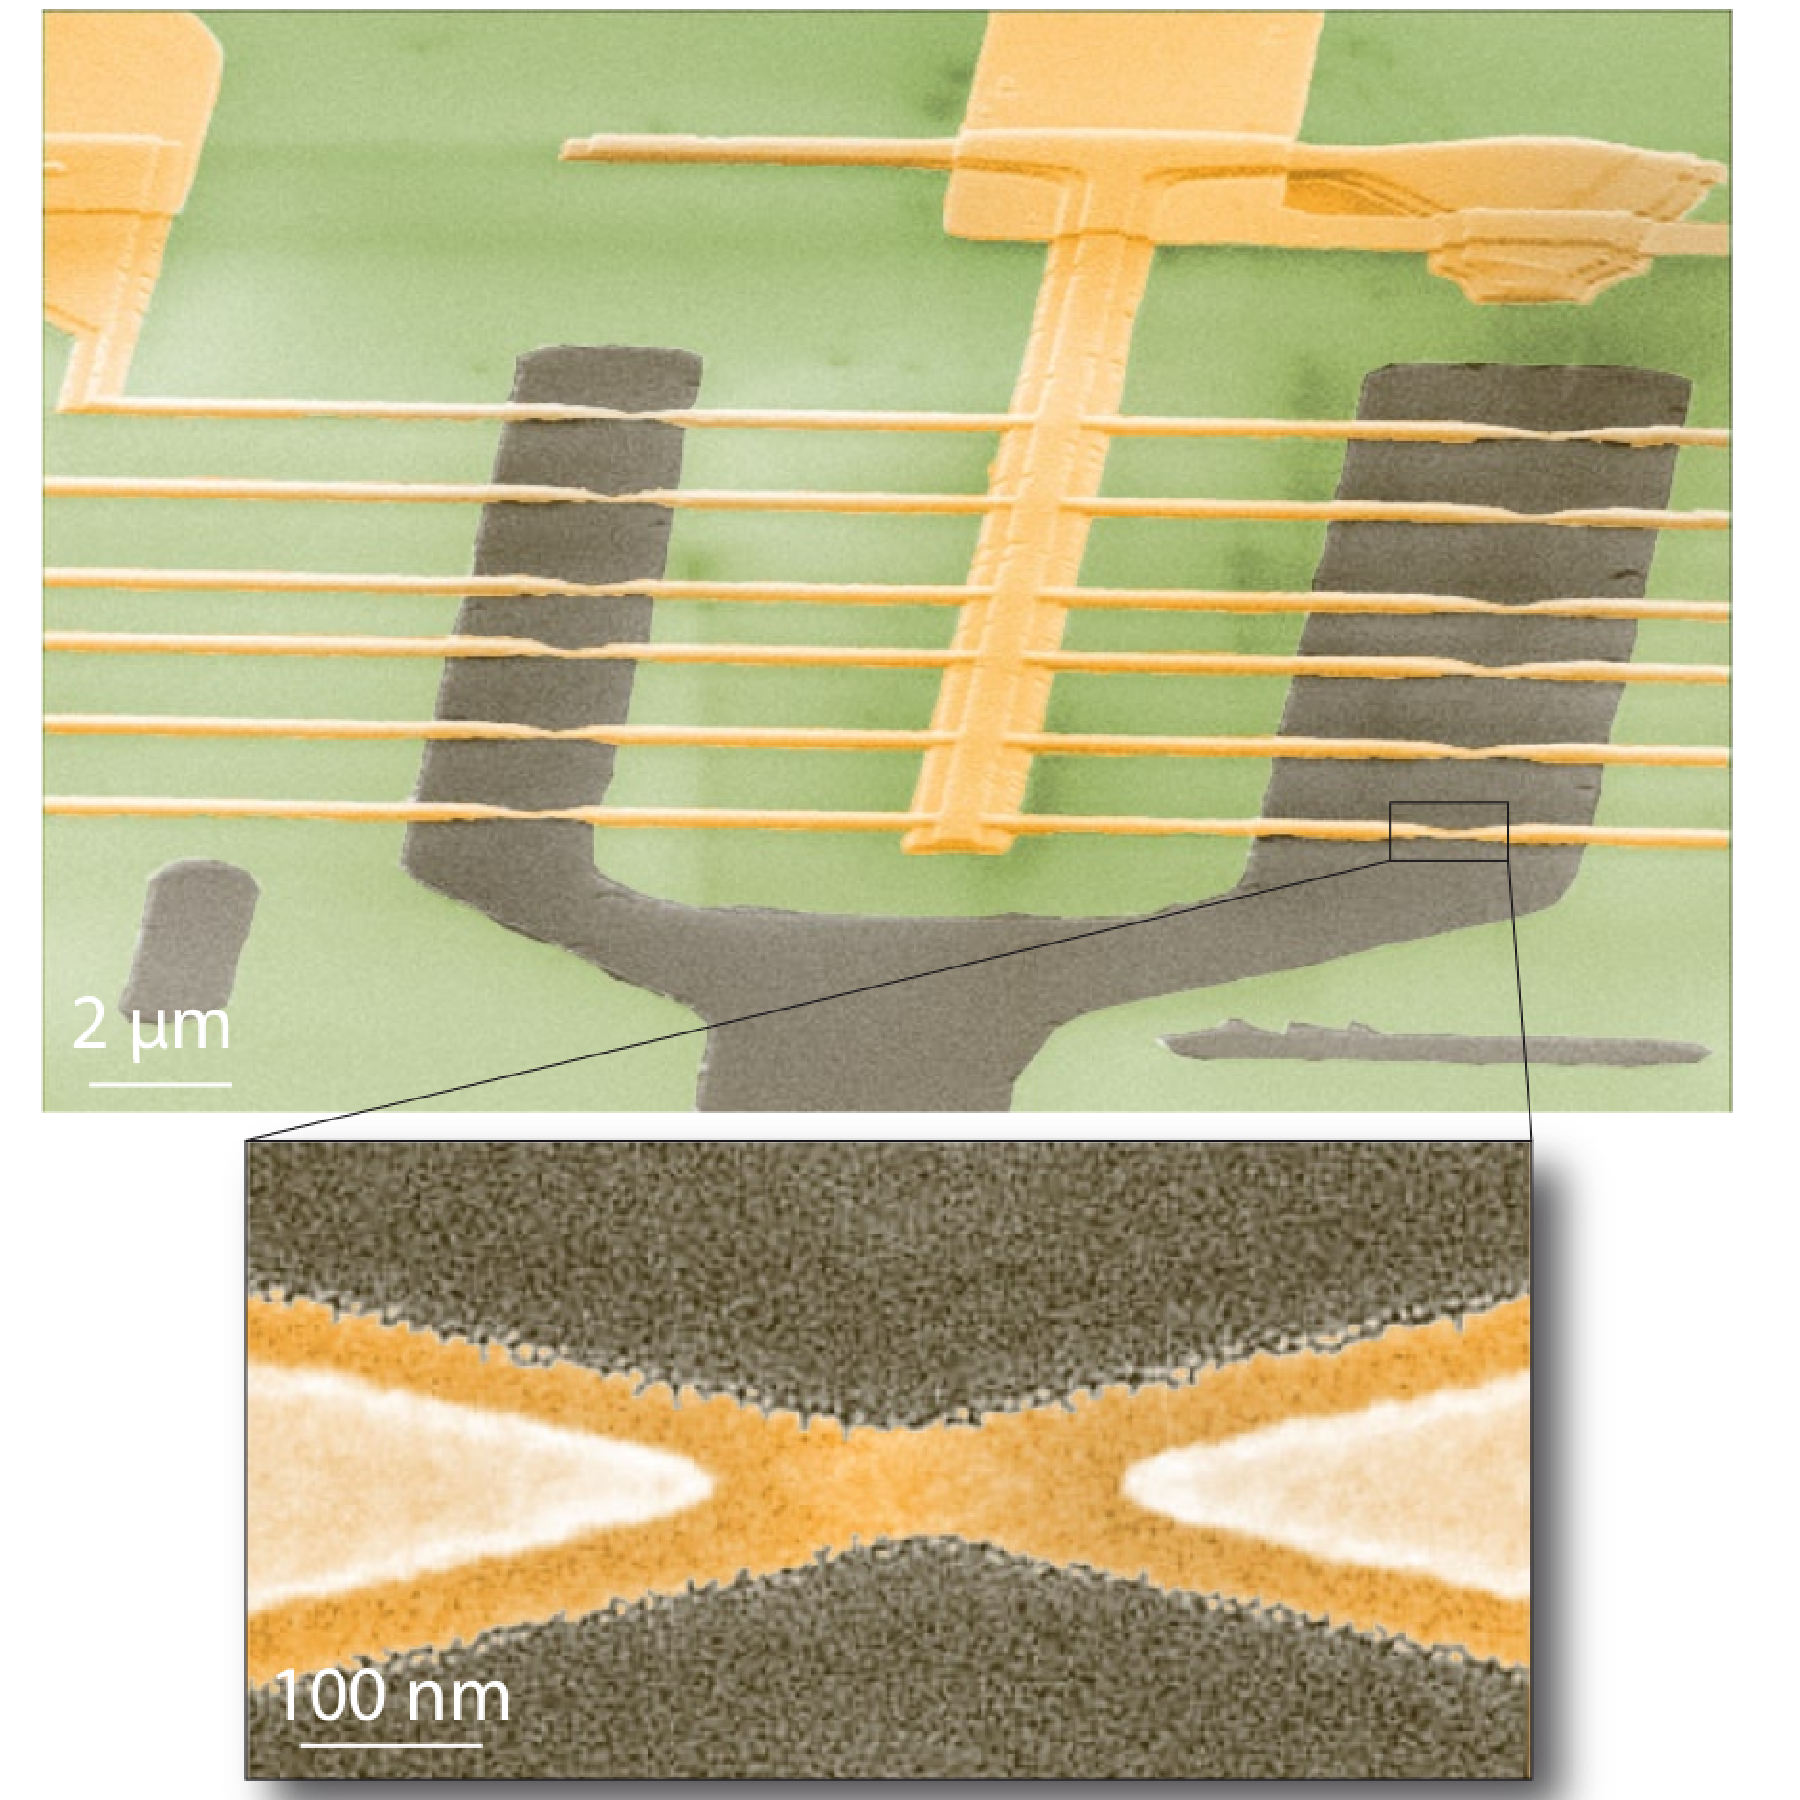
\includegraphics[scale=0.45]{Fabrication/ZoomFinal/ZoomFinal.pdf}
%\caption{Image obtenu par microscopie électronique à balayage montrant la structure centrale de nos échantillons. Le grossissement présente une constriction obtenue à l'aide de l'évaporation sous angle. La grille, colorée en gris, est clairement visible au centre (extrait de \cite{RochPhD}).}
%\label{ZoomFinal}
%\end{figure}


\section{Réalisation d'un interstice nanométrique}
Une fois que nous avons obtenu nos constrictions métalliques, il faut procéder à la dernière étape de fabrication : l'électromigration. Cette dernière, qui est effectuée à basse température, va nous permettre d'obtenir les interstices de quelques nanomètres de largeur, nécessaires à la fabrication d'un transistor moléculaire. Dans ce chapitre, nous présenterons dans un premier temps la technique d'électromigration ainsi que les différentes méthodes de mise en œuvre. Nous finirons par une description de notre technique de contre-réaction rapide à basse température.

\subsection{L'électromigration}
L'électromigration est un phénomène connu depuis plus d'un siècle maintenant~\cite{Gerardin1861}. Ce phénomène a connu un regain intérêt avec le développement de la micro-électronique, notamment parce qu'il a été identifié comme étant une cause de panne récurrente~\cite{Blech1967,Black1969}.

Il se produit lorsqu'une forte densité de courant traverse un conducteur. Les ions du réseau sont alors soumis à deux forces : la première est induite par le champ électrique générant le courant, la seconde est d\^u aux électrons qui, du fait de la diffusion, viennent céder un peu de leur moment cinétique~\cite{Ho1989}. L'action de ces deux forces se résume par la formule suivante :
\begin{eqnarray}
\textbf{F} = \textbf{F}_d + \textbf{F}_v = Z^*e\textbf{E} \nonumber
\end{eqnarray}
où $\textbf{F}_d$ est la force induite par le champ électrique et $\textbf{F}_v$ celle induite par la diffusion des électrons. Le terme $Z^*$ est en général utilisé pour représenter la charge effective des ions soumis à un champ électrique et rend compte de l'interaction ions/électrons.

Ce phénomène a été pour la première fois utilisé en électronique moléculaire par le groupe de D.C. Ralph à Cornell~\cite{Park1999}. La technique a notamment été mis en oeuvre pour réaliser le premier transistor à molécule unique~\cite{Park2000}. Depuis, elle a connu de nombreuses évolutions comme nous allons le voir maintenant

\subsection{Etat de l'art}
On peut classer les techniques d'électromigrations en trois grandes catégories : à rampe unique, à contre-réaction et à cassure-spontanée~\cite{Girod2012}.

\subsubsection{À rampe unique}
C'est la première technique a avoir été mise en œuvre dans le domaine de l'électronique moléculaire par Park \textit{et al.}~\cite{Park1999}. Elle consiste en l'application d'une rampe de tension croissante sur une fin fil de métal (voir Fig.\ref{ParkExemp}). La simplicité de la méthode est séduisante, mais mal contrôlée, elle peut conduire à une destruction de la jonction, notamment dû au chauffage induit par effet Joule.

\begin{figure}
\parbox{7cm}{
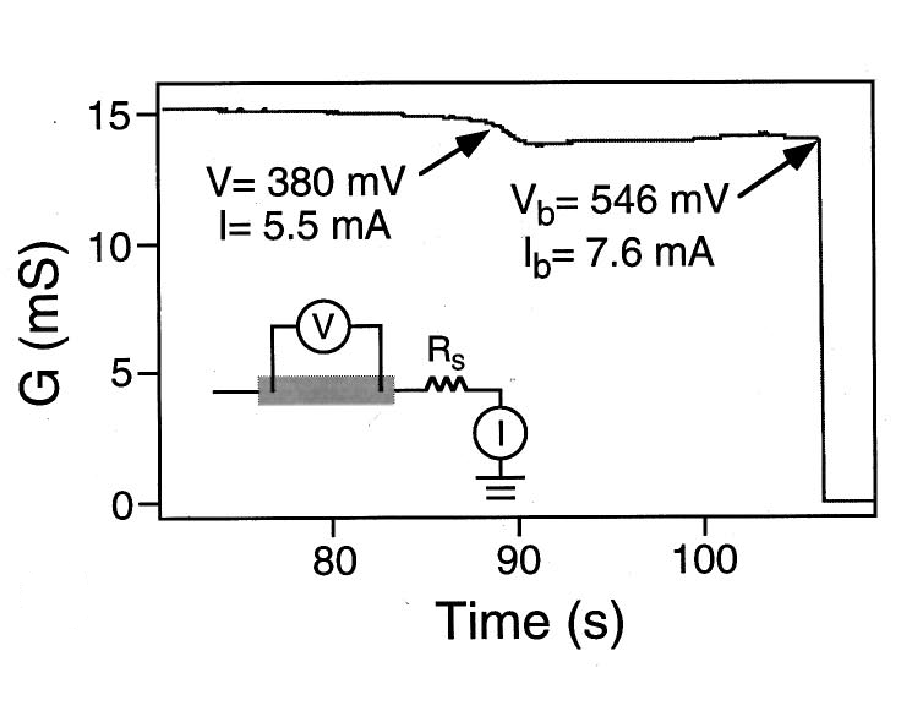
\includegraphics[scale=0.45]{Fabrication/ElecMigExemp/ParkFig.pdf} 
}
\parbox{5cm}{\caption{Evolution de la conductance d'un nanofil au court du temps lors d'une procédure d'électromigration à rampe unique. Extrait de~\cite{Park1999}.}
\label{ParkExemp}
}
\end{figure}



\subsubsection{À contre-réaction}
Cette méthode à été développée par Strachan \textit{et al.} en 2005~\cite{Strachan2005}. Elle a pour but de réduire le chauffage de la jonction par effet Joule~\cite{Esen2005} en introduisant une boucle de contre-réaction asservie sur la résistance de la jonction. Si celle-ci dépasse une valeur critique fixée à l'avance, la tension est diminué puis augmente à nouveau. Ceci à pour effet de réduire la puissance dissipée par la jonction lors de l'électromigration (voir Fig.\ref{EseExemp}). Le principal inconvénient de cette technique est son temps de mise en œuvre : la formation d'un seul gap peu prendre plusieurs heures.


\begin{figure}
\parbox{7cm}{
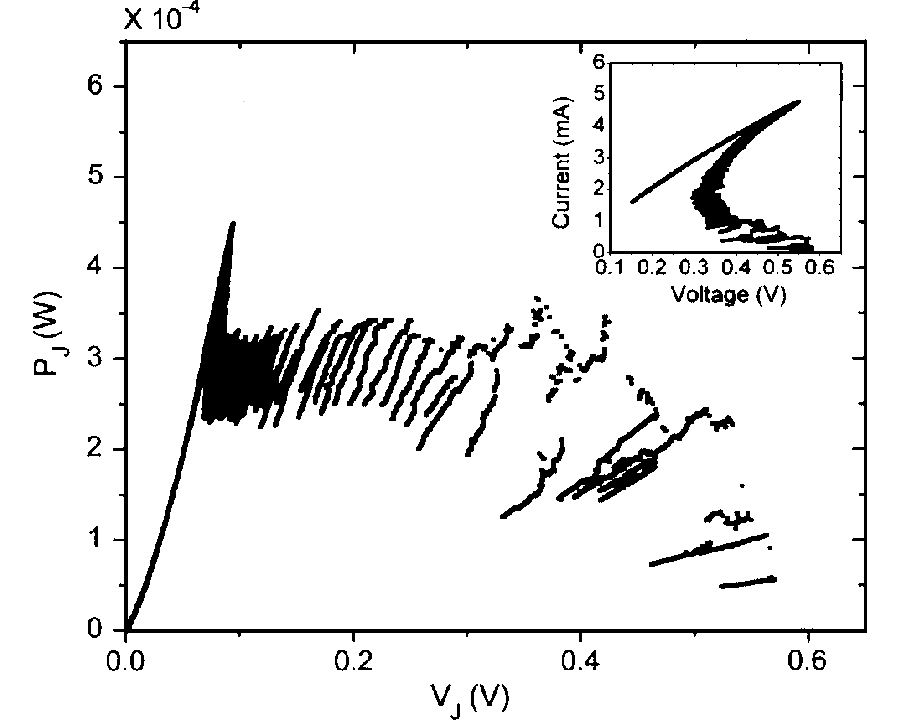
\includegraphics[scale=0.45]{Fabrication/ElecMigExemp/EseFig.pdf} 
}
\parbox{5cm}{\caption{Evolution de la puissance dissipée en fonction de la tension appliquée lors d'une procédure d'électromigration à contre-réaction. En encart, caractéristique courant-tension lors de cette m\^eme procédure. Extrait de~\cite{Esen2005}.}
\label{EseExemp}
}
\end{figure}


\subsubsection{À cassure spontanée}
Cette dernière méthode a été mise au point dans le groupe de H.S.J. van der Zant en 2007~\cite{ONeill2007}. Une première étape d'électromigration contrôlée est d'abord réalisée à l'aide d'une méthode à contre-réaction jusqu'à ce que la conductance du nanofil atteigne une valeur de quelques kilo-Ohms. On laisse ensuite évoluer la jonction qui, du fait de l'instabilité de la nanoconstriction, va se rompre naturellement. On obtient ainsi un gap de quelques nanomètres. La durée d'une telle procédure varie d'un échantillon à l'autres : de quelques minutes à plusieurs heures (voir Fig.\ref{ZantExemp}).

\begin{figure}
\parbox{7cm}{
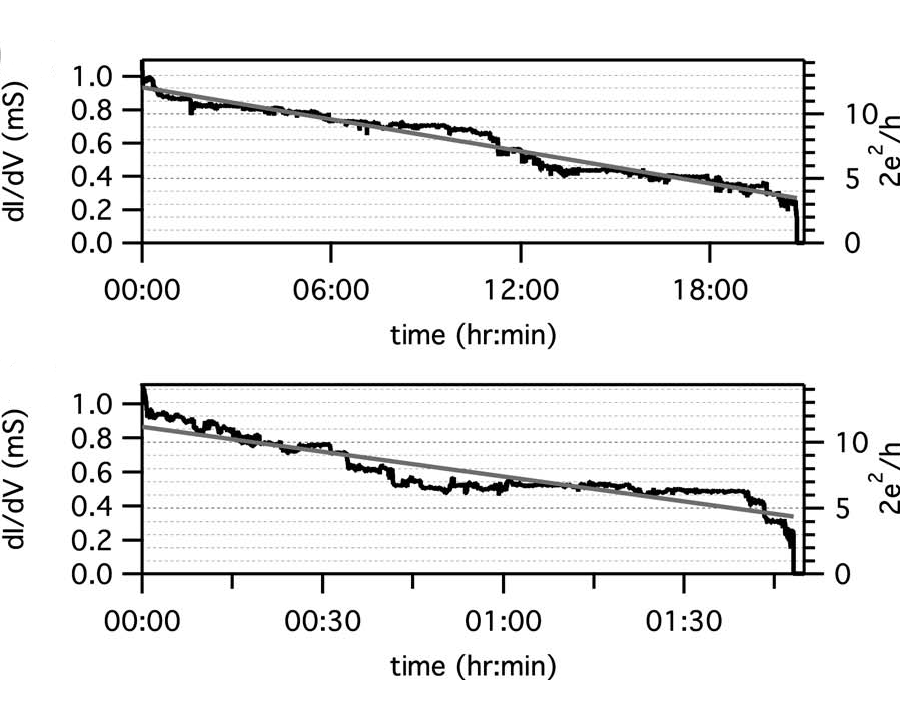
\includegraphics[scale=0.45]{Fabrication/ElecMigExemp/ZantFig.pdf} 
}
\parbox{5cm}{\caption{Évolution de la conductance de deux nanofils au cours du temps lors d'une procédure d'électromigration à cassure spontanée. Extrait de~\cite{ONeill2007}.}
\label{ZantExemp}
}
\end{figure}



\subsection{Notre technique}
Notre technique de fabrication a été développée à partir des travaux de Park \textit{et al.}~\cite{Park1999} puis améliorée en s'inspirant de travaux ultérieurs.

Afin d'augmenter le rendement de la méthode et la qualité des interstices obtenus, il a fallu apporter quelques modifications. Tout d’abord, la résistance en série avec la jonction à été diminuée au maximum~\cite{Zant2006,Trouwborst2006,Taychatanapat2007}. Cela permet de limiter la puissance dissipée au niveau de la jonction et donc de mieux contrôler l'électromigration.

\begin{figure}
\centering 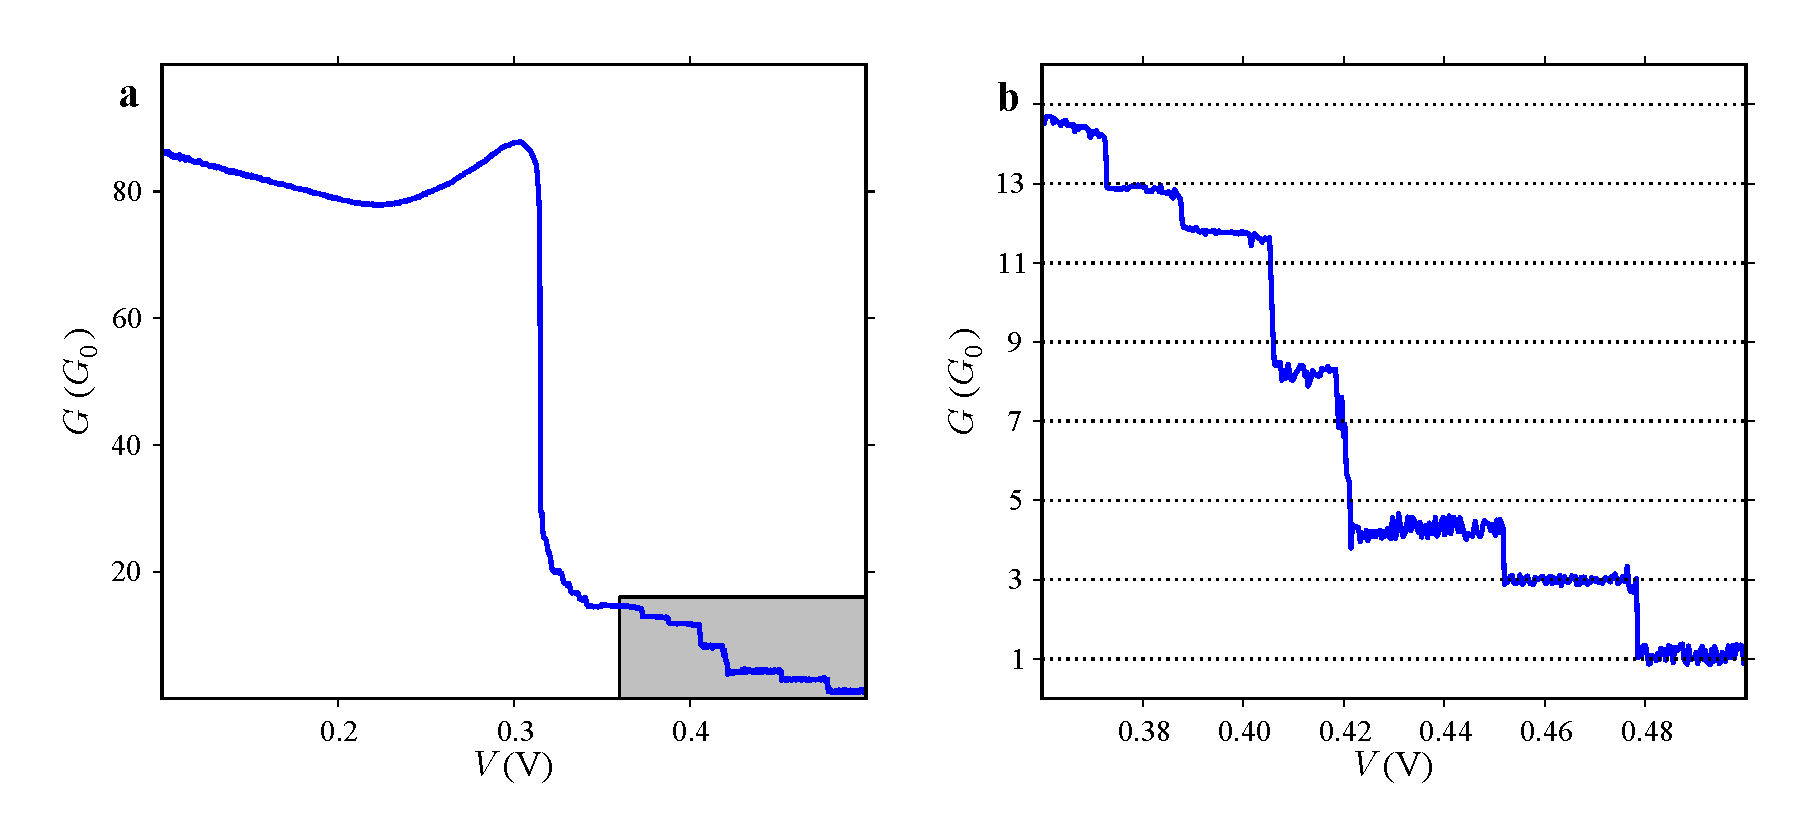
\includegraphics[scale=0.45]{Fabrication/NotreElectroMig/NotreElectroMig.pdf}
\caption{\textbf{a} : conductance de la jonction durant l'électromigration. \textbf{b} : grossissement de la partie grisée de \textbf{a} montrant les marches de conductance différentielle témoignant du bon déroulement de l'électromigration.}
\label{NotreElecMig}
\end{figure}


L'échelle de temps de l'électromigration est du domaine de la centaine de $\mu s$~\cite{ONeill2007}. Afin de pouvoir contrôler parfaitement le déroulement du phénomène, il faut être capable d'agir sur ce dernier en un intervalle de temps du même ordre. Ceci n'est possible que si la procédure d'électromigration se fait à l'aide d'une électronique en temps réel. Nous avons pour cela utilisé un ADWin contrôlé par le programme NanoQT, développé au sein du groupe. Grâce à ce dispositif, l'électromigration peut être détectée et la tension au borne de la jonction ramenée à zéro dans un intervalle de $10\, \mu s$.

De plus, l'étape d'électromigration se fait à $4\,K$ et sous atmosphère hélium ce qui prévient la contamination de l'interstice et permet d'analyser le dispositif obtenu directement après la procédure.

Ainsi, nous pouvons obtenir des interstices de la taille souhaitée ($\sim 1\,nm$) de façon reproductible. La Fig.\ref{NotreElecMig} présente la mesure en conductance lors d'un procédure d'électromigration. On observe trois régimes : dans un premier temps, la conductance diminue du fait de l'effet Joule; puis celle-ci augmente à nouveau du fait d'un réarangement de la jonction; enfin, la conductance chute brutalement et le phénomène d'électromigration commence. On peut notamment observer, en fin de procédure, les derniers plateaux de conductance, démontrant que l'électromigration est parfaitement contrôlée.


\section{Fabrication d'un transistor à molécule unique}
Pour obtenir un transistor moléculaire, il faut procéder selon trois étapes. La première consiste en la réalisation d'un nanofil reposant sur une grille. On dépose ensuite les molécules sur la puce avant de la micro-souder et de la disposer dans un frigo à dilution. Enfin, on procède à l'électromigration. Dans la partie précédente, nous avons abordé l'étape un et trois. Nous allons maintenant voir comment les molécules sont déposées ainsi que la technique de caractérisation électrique des interstices.

\subsection{Dép\^ot des molécules}
Les cristaux de TbPc$_{2}$ sont dissous dans du dichlorométhane à la concentration 10$^{-6}mol.L^{-1}$. Une goutte de la solution obtenue est ensuite déposée sur l'échantillon et séchée par un flux d'azote. L'échantillon obtenu est ensuite microsoudé sur le porte échantillon, disposé dans un frigo à dilution et électromigré à basse température. Les jonctions obtenues (jusqu'à 12 par échantillons) sont ensuite analysées en transport.

\subsection{Caractérisation des jonctions}
%La première analyse généralement effectuée consiste à mesurer la conductance du système en fonction de la tension de grille, pour une tension source-drain nulle. La présence d'un objet nanométrique fait apparaître un ou plusieurs pics que l'on nomme pics de Coulomb~\cite{Beenakker1991,Wiel2002,Hanson2007}~(cf annexe sur le transport mésoscopique). Si cette première analyse se révèle concluante, on procède à une étude plus fine à l'aide d'un diagramme de Coulomb dans lequel on trace la conductance différentielle en fonction de la tension de grille $V_{\rm{g}}$ et la tension source-drain $V_{\rm{ds}}$. On peut alors identifier trois régimes en fonction du coulage électronique entre l'objet situé dans l'interstice et les électrodes.
%
%\subsubsection{Couplage faible}
%Dans ce régime, la conductance mesurée est largement inférieur au quantum de conductance $G_0$~($\sim 72\,mS$). Cela se traduit par la présence de diamant de Coulomb aux bords très bien définis comme le montre la Fig.\ref{CouplageInt}.\textbf{a}. Ce faible couplage ne perturbe que légèrement les niveaux de l'îlot. Ils conservent donc leur élargissement intrinsèque, d'où la finesse des bords de diamant. Dans cette configuration, seul le tunneling séquentiel est responsable du courant circulant à travers le système. Si l'on désire explorer les propriétés intrinsèques de l'îlot, le couplage faible est le régime idéal.
%
%\subsubsection{Couplage intermédiaire}
%Lorsque la conductance du système est proche du quantum de conductance, le couplage est qualifié d'intermédiaire. De nouveaux processus de transport peuvent alors être observés comme le cotunneling par exemple. Ce régime est notamment observé dans la Fig.\ref{CouplageInt}.\textbf{b} où des variations de conductance à l'intérieur même des diamants de Coulomb sont mesurés. Celle-ci correspondent à des processus du second ordre permettant aux électrons de circuler, même lorsque le système se trouve en régime de blocage de Coulomb~(Pour plus de détail, le lecteur peut se référer à l'annexe sur le transport mésoscopique). Ce régime entraîne également un élargissement des niveaux de l'îlot central du fait de la forte hybridation de ces derniers avec les niveaux électronique de la source et/ou du drain.
%
%\begin{figure}
%\centering 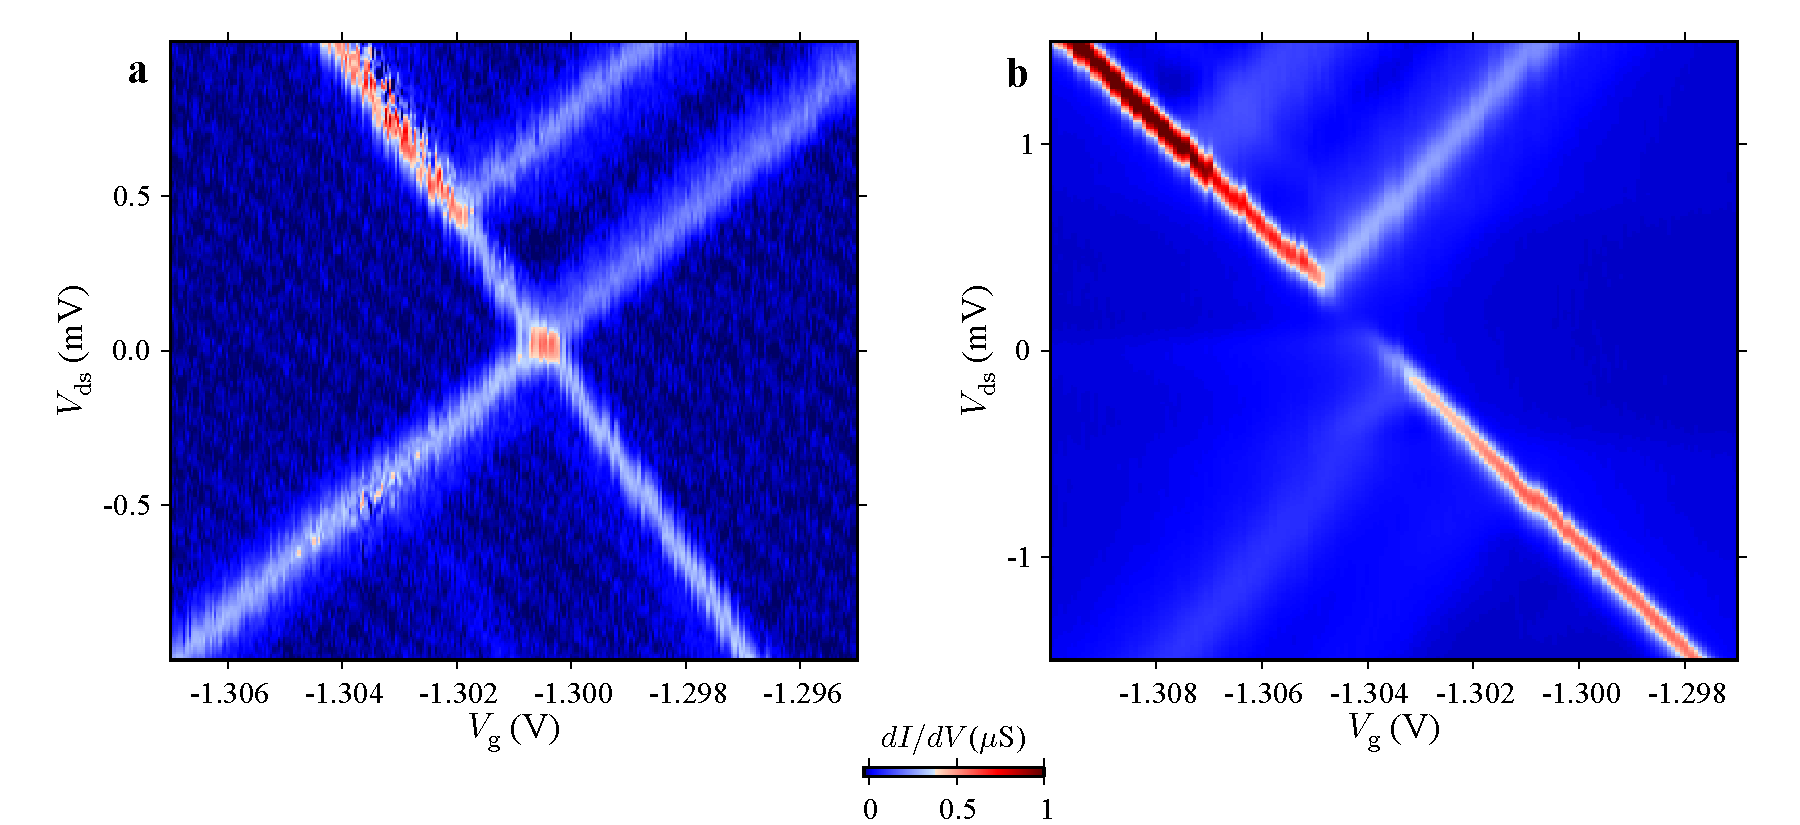
\includegraphics[scale=0.45]{Fabrication/CouplageInt/CouplageInt.pdf}
%\caption{\textbf{a} : diamant de Coulomb correspondant à un couplage faible. Les bords de diamants sont bien définis et aucune ligne de cotunneling n'est présente. \textbf{b} : diamant de Coulomb correspondant à un couplage intermédiaire. Les bords de diamant reste bien définie mais des lignes de cotunneling sont clairement visible à l'intérieur du régime de blocage.}
%\label{CouplageInt}
%\end{figure}
%
%
%\subsection{Couplage fort}
%Lorsque l'hybridation des niveaux est telle qu'ils deviennent indiscernables, le couplage est qualifié de fort et les propriétés intrinsèques de l'îlot central sont fortement altérées. En général, ce régime est présent lorsque la conduction ou, autrement dit, le taux d’événements tunnels $\Gamma$ est plus grand que l'énergie séparant deux états de charge de l'îlot.
%
%Ce régime est à éviter si l'on souhaite étudier les propriétés intrinsèque de l'\^ilot central.
